%##########################  CHAPER 6: APPLICATION  #######################

\chapter{Entwicklung der Anwendung}\label{kap:application}

Dieses Kapitel beschreibt die Entwicklung der Anwendung, als 
autonomes System welches auf dem Raspberry Pi läuft, 
Bilder über eine infrarotfähige Kamera aufnimmt und diese
auf dem Neural Compute Stick 2 mit dem trainierten Modell 
inferiert.
Desweiteren wird die Implementierung der verbindugn zu einem 
Host Pc beschrieben.


%-------------------------  SECTION 1: AUFBAU  ------------------------
\section{Aufbau/Hardware}\label{sec:aufbau}



Der Anwendungs Code läuft auf dem Raspberry Pi, an den 
der Neural Compute Stick über eine Usb Schnittstelle 
angeschlossen wird.
Das ausführen der Inferenz uf dem MYRIAD Chip des NCS2 
wird in der Implementierung der InferenceEngine festgelegt.

Bei der verwendeten Kamera handelt es sich um ein Raspberry Pi 
Kamera Modul mit 5MP OV5647 Sensor 
und automatschem umschalten der Infrarot Funktion der Marke 
Longrunner. (CSI-Schnittstelle (Camera Serial Interface) )
%https://www.amazon.de/gp/product/B07R4JH2ZV/ref=ppx_yo_dt_b_asin_title_o01_s00?ie=UTF8&psc=1
Dieses verfügt zusätzlich über zwei Infrarot LEDs, mit 850 nm wellenlänge.
Für das Umschalten in den Infrarot Modus, wird der Infrarot Filder, welcher sich 
für normale Aufnahmen vor der Linse befindet entfern, was über einen magnetschalter 
der über einem Helligkeitssensor getriggert wird erfolg.

\begin{minipage}{0.55\textwidth}
    \centering
    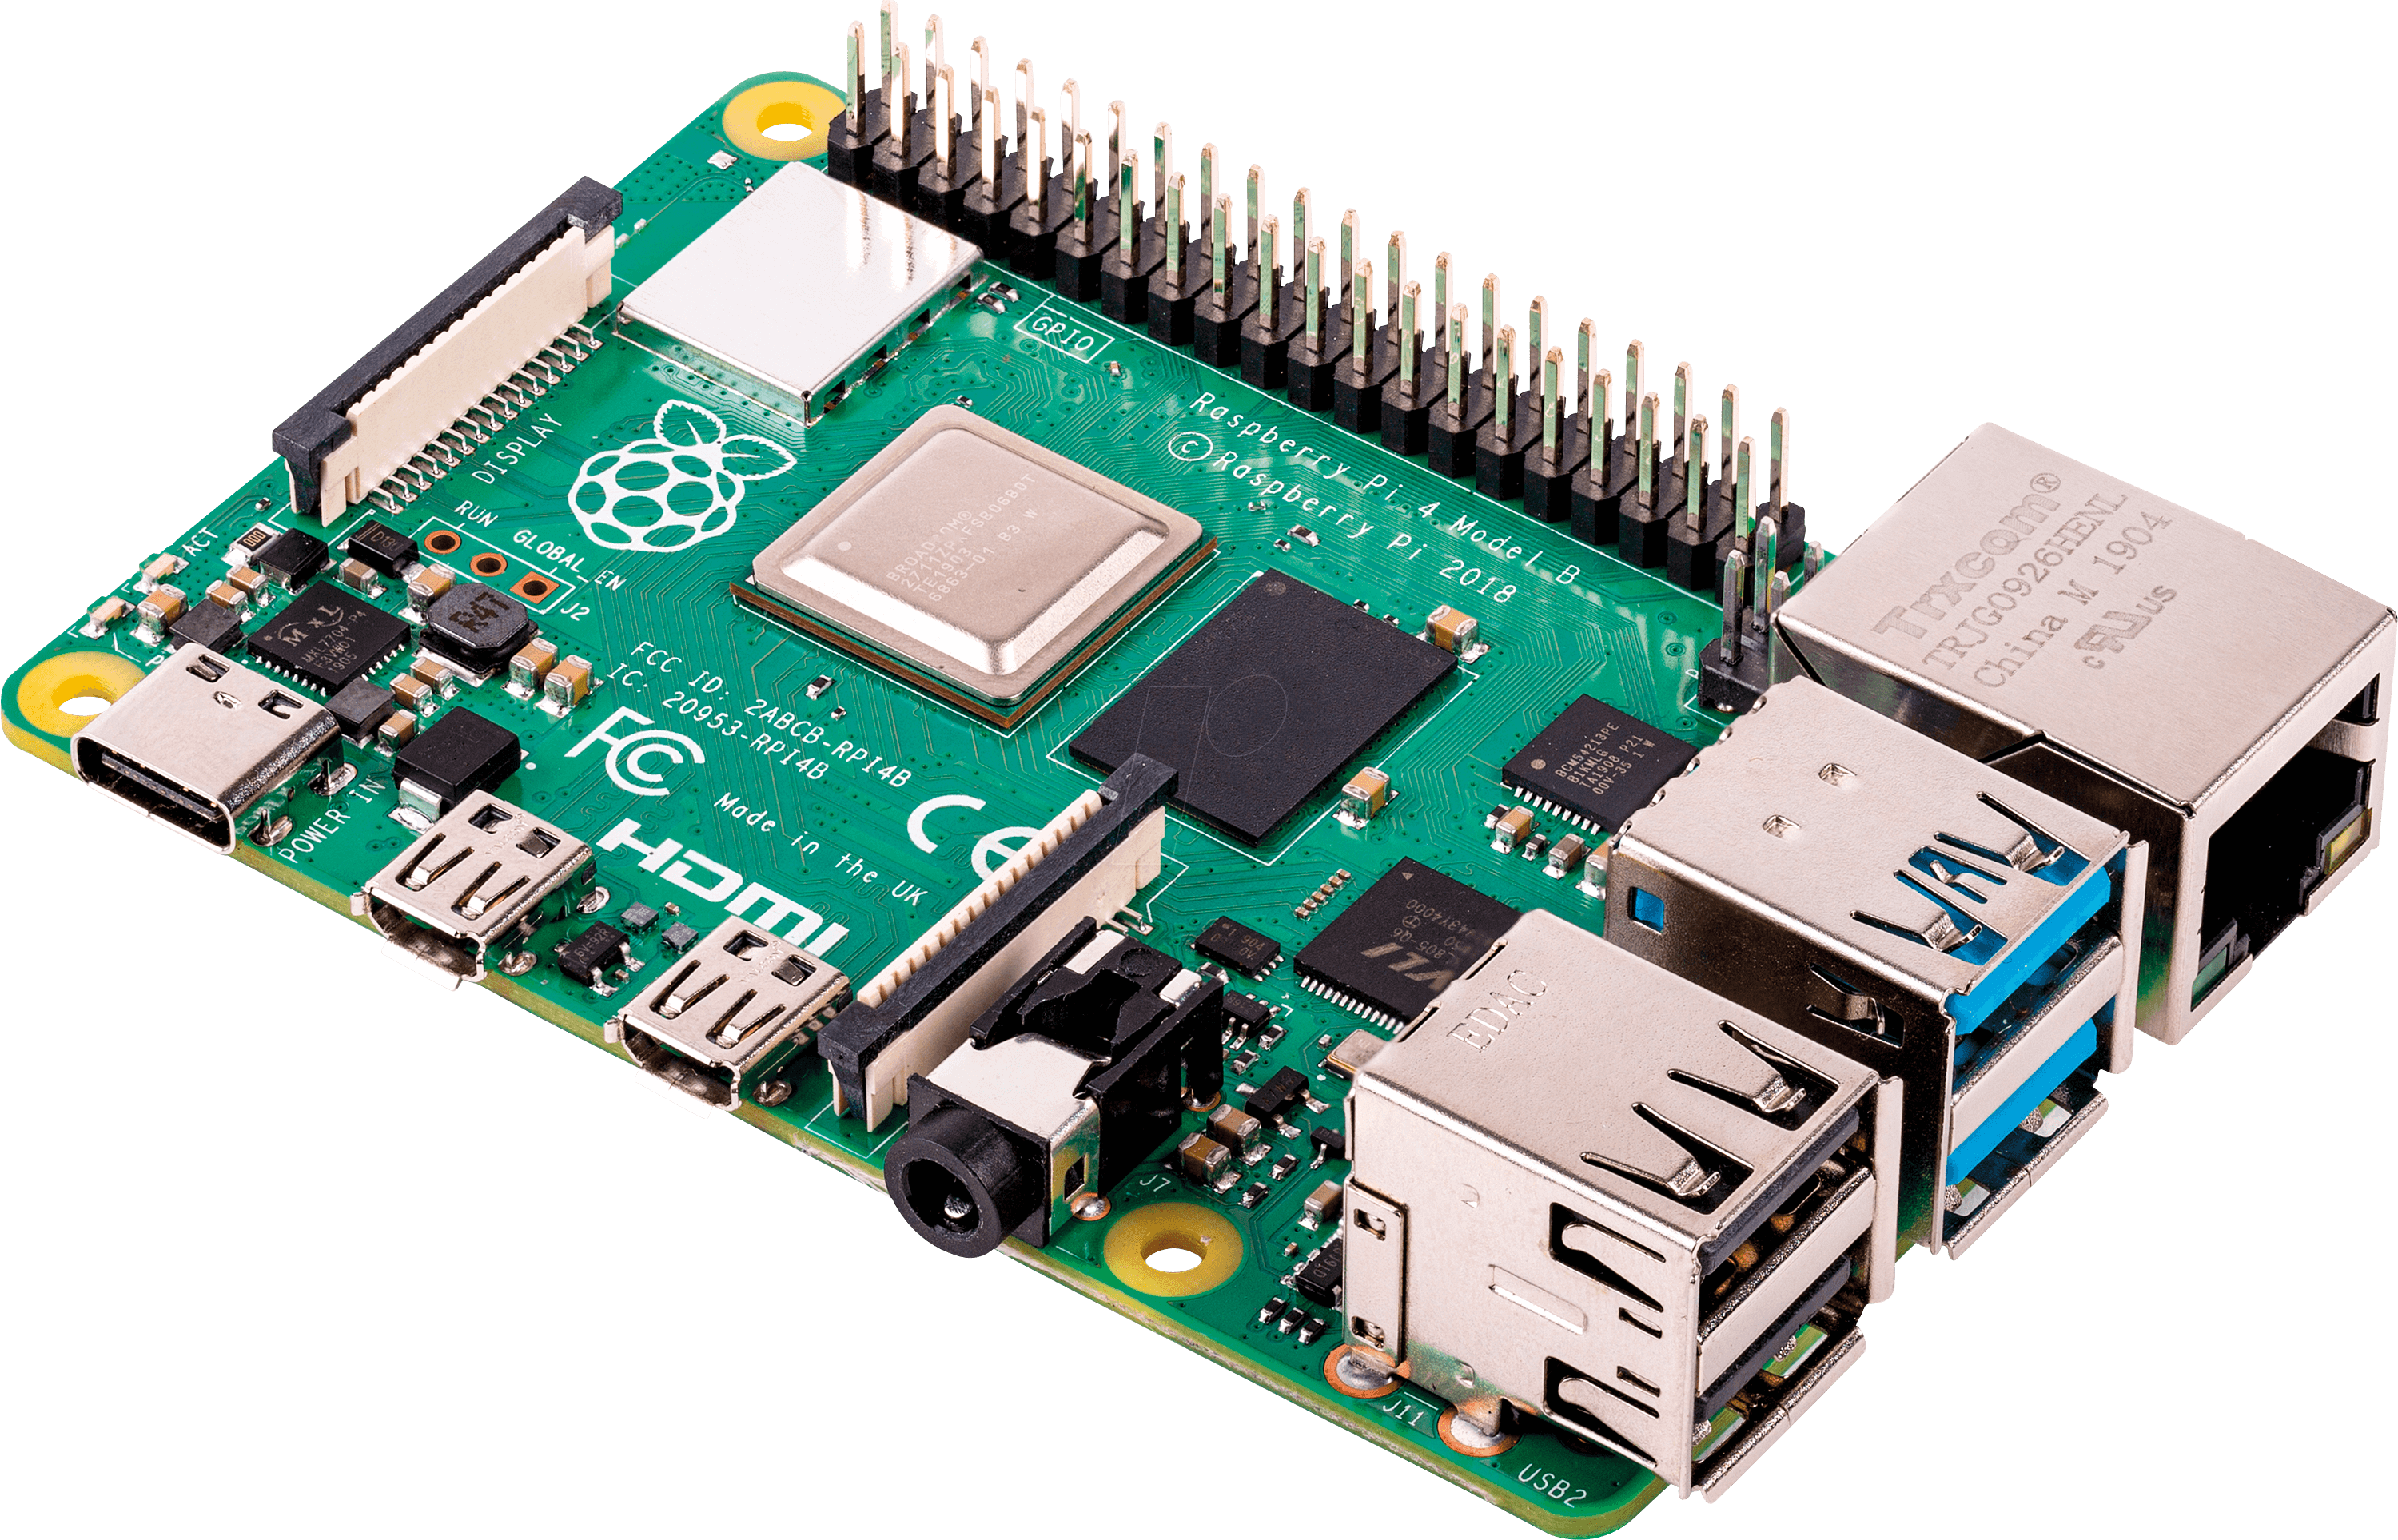
\includegraphics[width=0.8\textwidth]{./Bilder/raspberrypi_4.png}
    \captionof{figure}{Raspberry Pi 4}
    \label{img:raspberrypi}
\end{minipage}
\begin{minipage}{0.45\textwidth}
    \centering
    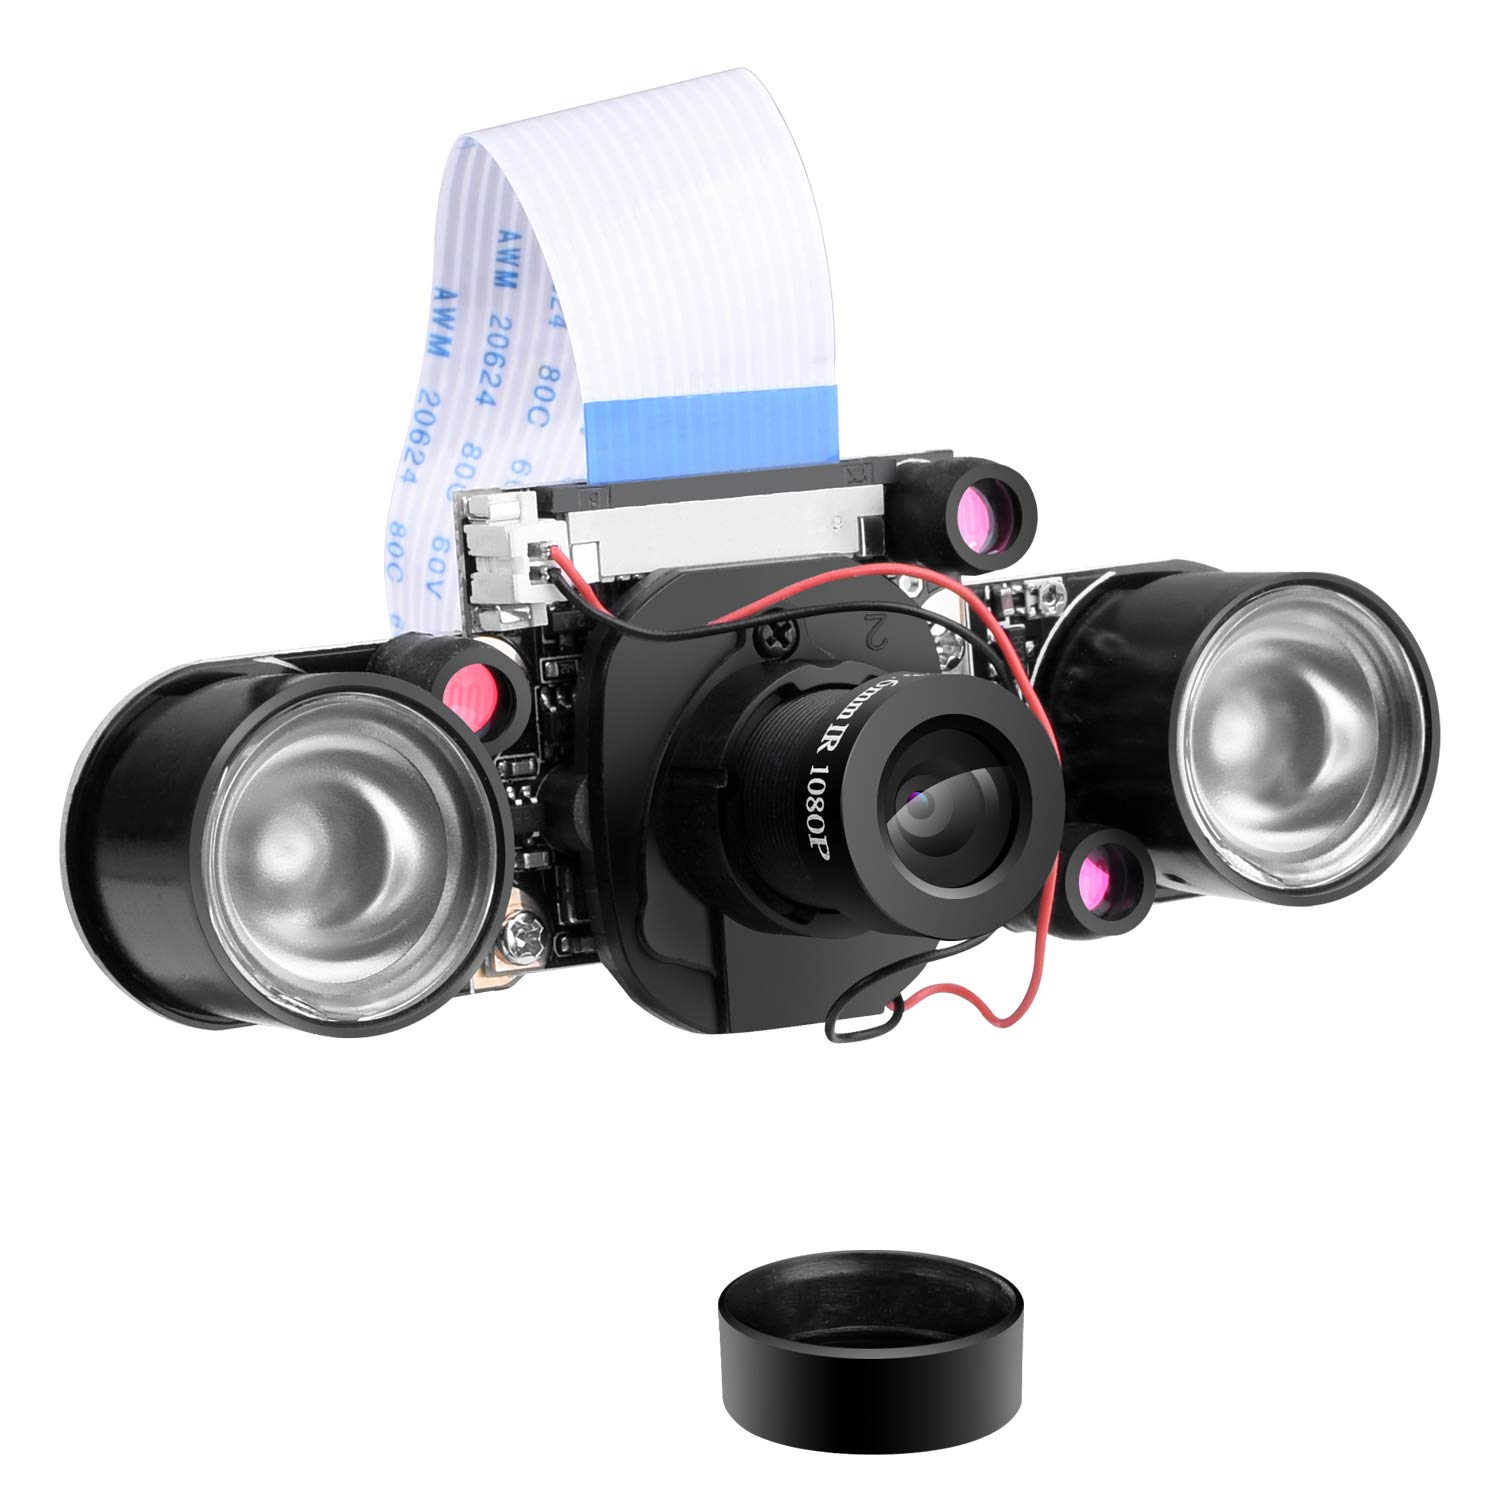
\includegraphics[width=0.8\textwidth]{longrunner.jpg}
    \captionof{figure}{Longruner Kamera Modul}
    \label{fig:rpicam}
\end{minipage}
\vspace{0.6cm}


Desweiteren wurde für eine mobile Internetverbindung 
der \textit{Huawei E3531 SurfStick} und zu Stromversorgnung
eine Powerbank verwendet.


% https://www.amazon.de/gp/product/B00HSZEY34/ref=ppx_yo_dt_b_asin_title_o00_s00?ie=UTF8&psc=1


\section{Implementierung/Software}

Main Programm verwendet folgende drei Klassen.

% \input{Bilder/class_diagramm/class_diagramm.latex}

% \begin{minipage}{0.3\textwidth}
%     \centering
%     \input{Bilder/diagramme/class_detection.tex}    
% \end{minipage}
% \begin{minipage}{0.3\textwidth}
%     \centering
%     \input{Bilder/diagramme/class_connection.tex}
% \end{minipage}
% \begin{minipage}{0.3\textwidth}
%     \centering
%     \input{Bilder/diagramme/class_motion.tex}
% \end{minipage}

% oder

%\input{Bilder/diagramme/detection_package.tex}

% oder 

\vspace{1cm}

\begin{tikzpicture} 

    
    
            \umlclass{Motion}{ 
              statickBackground : np.array
              }{ 
              + detectMotion() : bool \\
              + resetBackground() : void
            }
        
            \umlclass[y=-4]{InferenceModel}{ 
                string : plugin
                strin : device
                }{ 
                + createExecInferModel() : ExecInferModel
              }
        
            \umlclass[y=-2, x=6]{ExecInferModel}{ 
                shape : ioBlob\\
                detected : array
                }{ 
                + inferFrames() : status \\
                \# status[0] num infered\\
                \# status[1] num detected\\
                \# status[2] num saved\\
                - save() : void
                }
        
    
        \umlclass[x=11, y=-2]{Connection}{ 
            string logindata
            }{ 
            + login() : bool \\
            + connect() : server, port\\
            + send() : bool\\
            + disconnect() : bool\\
            + sendEmail(email, text) : boiol
          }

    
    \end{tikzpicture}
        




\subsection*{Inferenz}


Um nicht durchgehend die Input Frames welche die Kamera liefert inferieren zu 
müssen, wurde mithilfe der Library OpenCV ein bewegungserkennung 
implementiert. Diese speichert bei start der Anwendung ein Frame 
als Refernz ab, und kann damit alle weiteren Input frames vergleiche, 
indem der Abstand der einzelnen Pixel werte berechnet und gemittelt wird.

Der Ablauf der reinen Asynchronen Inferenz ist grob in 
folgendem Pseudocode dargestellt. 


%Asynchrone inferenz
%https://docs.openvinotoolkit.org/latest/_demos_python_demos_object_detection_demo_ssd_async_README.html

% main
% \begin{algorithm}[H]
%     \caption{Main Program}
%     \begin{algorithmic}

%     %\STATE INIT EXEC_NET, CAM

%     \WHILE{\TRUE}
%         \STATE capture frame
        
%         \IF{frame has motion}
%             \STATE $buffer \leftarrow frmae$
%         \ENDIF

%         \IF{buffer is empty}
%             \STATE disconnect
%         \ENDIF

%         \STATE result = inferFrames (buffer)

%         \FOR{all results}
%             \STATE process results
%             \IF {saved}
%                 \STATE sendRequest = \TRUE
%             \ENDIF
        

%             \IF {no detectoin for 20 times}
%                 \STATE reset motion background
%                 \STATE delete buffer
%                 \IF {connected}
%                     \STATE disconnect
%                 \ENDIF
%             \ENDIF

%         \ENDFOR

%         \IF {send all every minute}
%             \STATE save current detections
%             \STATE sendRequest = \TRUE
%         \ENDIF

%         \IF{sendRequest == \TRUE}
%             \IF{not logged in}
%                 \STATE log in
%             \ENDIF

%             \IF{not connected}
%                 \STATE connect
%             \ENDIF

%             \STATE server, port $\leftarrow$ connection

%             \STATE sendRequest = \FALSE
%             \FOR{all saved images}
%                 \IF{send image $\rightarrow$ server, port}
%                     \STATE delete image
%                 \ELSE
%                     \STATE sendRequest = \TRUE
%                 \ENDIF
%             \ENDFOR

%         \ENDIF
%     \ENDWHILE


%     \end{algorithmic}
% \end{algorithm}

\begin{center}
    \rule{0.8\textwidth}{0.4pt}
    \begin{lstlisting}[language=Python]
        def infer_frames(Buffer, threshhold):
            for idx, inferRequest in all inferRequests:
                status = inferRequest.wait(0) # nicht blockierend
                if status not ready:
                    continue
                
                if idx in currentFrames:
                    results = inferRequest.output
                    frame = currentFrames[idx]

                if Buffer not empty:
                    currentFrames[idx] = Buffer.pop()
                    infer_frame = preprocess(currentFrames[idx])
                    inferRequest.async_infer(infer_frame)

                if results or frame is None:
                    continue

                for obj in all results:
                    Class, Roi, Proba <- obj
                    if Proba < threshhold:
                        continue
                    
                    coords <- Roi, frame.shape

                    infered_frame = draw_rect(frame, coords)

                    if proba > detectedObjects.proba
                        replace detectedObjects

                    if number of detections > x:
                        send(frame)
                    
    \end{lstlisting}
    \rule{0.8\textwidth}{0.4pt}        
\end{center}


% \centering\rule{0.6\textwidth}{0.4pt}
% \begin\centering{lstlisting}[language=Python]
%     def infer_frames():
%         for all requests:
%             do something \textbf{with} request

%             status = request.wait(0)
%             if status == done:
%                 res = requests.output
%                 frame = current[id]
% \end{lstlisting}
% \centering\rule{0.6\textwidth}{0.4pt}




% inferenz
\begin{algorithm}[H]
    \caption{Asynchrone Inferenz}
    \begin{algorithmic}
    \WHILE{\TRUE}
        \STATE capture Frame
        \IF{Frame has Motion}
            \STATE Buffer $\leftarrow$ Frame
        \ENDIF
        \FOR{$reqId$ = 0 to $reqMax$}
            \IF {Model.reqests[$reqId$].wait(0)}
                \STATE result = Model.reqests[$reqId$].output
                \STATE inferedFrames $\leftarrow$ (result, currentFrames[$reqId$])
                \IF {Buffer not empty}
                    \STATE currentFrames[$reqId$] $\leftarrow$ Buffer 
                    \STATE inFrame = preprocess: currentFrames[$reqId$]
                    \STATE Model.inferAsync($reqId$, inFrame)
                \ENDIF
            \ENDIF
        \ENDFOR
        \RETURN inferedFrames
    \ENDWHILE
    \end{algorithmic}
\end{algorithm}

wobei die wait Funktion mit Timeout = 0 nicht blockierend ist.

Dadurch war es möglich trotz langsamerer inferenz zeit als 
capture zeit, durch zwischenspeichern alle frames zu inferieren, 
unter der Annahme, das nur zeitweise bewegung erkannt und damit 
inferiert werden muss.



\subsection*{Connection}

\begin{itemize}
    \item remote Proxy verbinung über SSH
    \item mit SCP Protokol send
\end{itemize}

\newpage
\subsection{all}

\tikzset{
    desicion/.style={
        diamond,
        draw,
        text width=4em,
        text badly centered,
        inner sep=0pt
    },
    block/.style={
        rectangle,
        draw,
        text width=10em,
        text centered,
        rounded corners
    },
    arrow/.style={
        draw,
        >=latex,
        ->
    }
}


\begin{tikzpicture}
    \node (A) [desicion] {entschei\\dung};
    \node (B) [block, below of=A, node distance=3cm, text width=5em] {bock};
    \node (C) [block, right of=A, node distance=0.5\textwidth] {noch ein\\bock};


    \draw[arrow] (A) --  node [left, fill=white!30] {yes} (B);
    \draw[arrow] (A) -- node [below, near end] {crap} (C); 
    \draw[arrow] (B) -| node [near start, fill=white] {yes} (C);

\end{tikzpicture}


\newpage

%\tikzset{
    desicion/.style={
        diamond,
        draw,
        text width=4em,
        text badly centered,
        inner sep=0pt
    },
    block/.style={
        rectangle,
        draw,
        text width=5em,
        text height=1em,
        text centered
    },
    arrow/.style={
        draw,
        >=latex,
        ->
    }
}


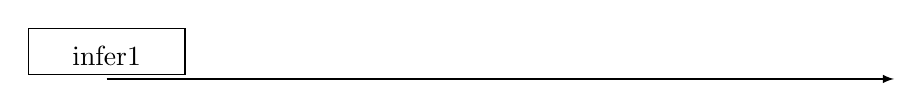
\begin{tikzpicture}

    \node(infer1) [block] {infer1};
    \draw[arrow] (0,-1em) -- (10,-1em);
    % \node (A) [desicion] {entschei\\dung};
    % \node (B) [block, below of=A, node distance=5cm, text width=5em] {bock};
    % \node (C) [block, right of=A, node distance=5cm] {noch ein\\bock};


    % \draw[arrow] (A) --  node [left, fill=white] {yes} (B);
    % \draw[arrow] (A) -- node [below, near end] {crap} (C); 
    % \draw[arrow] (B) -| node [near start, fill=white] {yes} (C);

\end{tikzpicture}


\begin{figure}[H]
    \centering
    \def\svgwidth{0.8\textwidth}
    \tikzset{
    desicion/.style={
        diamond,
        draw,
        text width=4em,
        text badly centered,
        inner sep=0pt
    },
    block/.style={
        rectangle,
        draw,
        text width=5em,
        text height=1em,
        text centered
    },
    arrow/.style={
        draw,
        >=latex,
        ->
    }
}


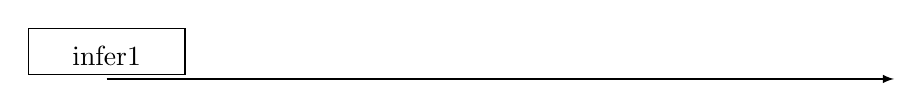
\begin{tikzpicture}

    \node(infer1) [block] {infer1};
    \draw[arrow] (0,-1em) -- (10,-1em);
    % \node (A) [desicion] {entschei\\dung};
    % \node (B) [block, below of=A, node distance=5cm, text width=5em] {bock};
    % \node (C) [block, right of=A, node distance=5cm] {noch ein\\bock};


    % \draw[arrow] (A) --  node [left, fill=white] {yes} (B);
    % \draw[arrow] (A) -- node [below, near end] {crap} (C); 
    % \draw[arrow] (B) -| node [near start, fill=white] {yes} (C);

\end{tikzpicture}

    \caption{}
    \label{}
\end{figure}

\vspace{2cm}

